
\documentclass[a4paper,12pt]{article}
\date{}

%-----------------------------------------------------------------------------
% Language setting, set page size and margins
%-----------------------------------------------------------------------------
\usepackage[english]{babel}
\usepackage[a4paper,top=2.5cm,bottom=2.5cm,left=2.5cm,right=2.5cm,marginparwidth=1.75cm]{geometry}
\usepackage{setspace}
\onehalfspacing %interligne 1.5
%----------------------------------------------------------------------------

% Useful packages
\usepackage{amsmath}
\usepackage{amssymb}
\usepackage{graphicx}
\usepackage[hidelinks]{hyperref}
\usepackage{subfigure}
%\usepackage[colorlinks=true, allcolors=blue]{hyperref}

%----------------------------------------------------------------------------
% Packages: uncomment to debug
%----------------------------------------------------------------------------
\usepackage{refcheck}
\renewcommand{\labelitemi}{\textbullet}

%----------------------------------------------------------------------------
% Packages: bibliography
%----------------------------------------------------------------------------
\usepackage[nottoc, notlof, notlot]{tocbibind}
%\usepackage[square,sort,comma,numbers]{natbib}
\usepackage[authoryear]{natbib}
%\usepackage[english]{babel}
\usepackage{authblk}

%----------------------------------------------------------------------------
% Acronyms
%----------------------------------------------------------------------------
\usepackage[acronyms]{glossaries}
\makeglossaries
%\newacronym{Identifiant unique}{Nom de l’acronyme}{Définition de l’acronyme}
\newacronym{kh}{KH}{Kelvin-Helhmoltz}

%----------------------------------------------------------------------------
% Page de garde
%----------------------------------------------------------------------------
\usepackage[utf8]{inputenc}
\usepackage[T1]{fontenc}
%\usepackage{fullpage}
\usepackage{eso-pic}
\newcommand{\HRule}{\rule{\linewidth}{0.5mm}}
\newcommand{\blap}[1]{\vbox to 0pt{#1\vss}}
\newcommand\AtUpperLeftCorner[3]{%
  \put(\LenToUnit{#1},\LenToUnit{\dimexpr\paperheight-#2}){\blap{#3}}%
}
\newcommand\AtUpperRightCorner[3]{%
  \put(\LenToUnit{\dimexpr\paperwidth-#1},\LenToUnit{\dimexpr\paperheight-#2}){\blap{\llap{#3}}}%
}

\title{ \Large{Rapport de Stage M2 SOAC-DC}}
\author{Marie Andrieux}
\makeatletter

%----------------------------------------------------------------------------
%----------------------------------------------------------------------------
%----------------------------------------------------------------------------
%                           BEGIN DOCUMENT
%----------------------------------------------------------------------------
%----------------------------------------------------------------------------
%----------------------------------------------------------------------------

\begin{document} 
%\maketitle
\thispagestyle{empty}

%----------------------------------------------------------------------------
% \ref with ( )
%----------------------------------------------------------------------------
\let\noparref\ref
\renewcommand{\ref}[1]{(\noparref{#1})}


%----------------------------------------------------------------------------
% Page de garde
%----------------------------------------------------------------------------
\begin{titlepage}
    \enlargethispage{2cm}
 
    \AddToShipoutPicture{
        %\AtUpperLeftCorner{1.5cm}{1cm}{\includegraphics[width=4cm]{figures/logolegos.jpg}}
        %\AtUpperRightCorner{1.5cm}{1cm}{\includegraphics[width=6.5cm]{data/logola.jpg}}
        }
 
    \begin{center}
        \vspace*{10cm}
        \textsc{\@title} \\
        \newline
        \large{\bf Influence de la diffusion moléculaire sur le mélange de traceurs passifs}
        \HRule
        \vspace*{0.5cm}
        \large{\@author} \\
        \newline
        \small{Tuteurs : Yves Morel (Legos), Francis Auclair (Laero) et Cyril Nguyen (Laero)}
        
    \end{center}
 
    \vspace*{9.2cm}
 
    \begin{center}
        %\makebox[\textwidth]{\includegraphics[width=\paperwidth]{figures/???}}
    \end{center}
 
\end{titlepage}
\ClearShipoutPicture

\newpage
%----------------------------------------------------------------------------
% Page numbering
%----------------------------------------------------------------------------
\renewcommand{\thepage}{\arabic{page}}
\setcounter{page}{1}


%----------------------------------------------------------------------------
%%  ABSTRACT
%----------------------------------------------------------------------------
\begin{abstract}
25 à 30 pages maximum dont le contenu indicatif est le suivant : 1 résumé, 1 table des matières, 1 liste des acronymes si nécessaire, 1 introduction (posant la problématique, restituant les questions abordées dans leur contexte scientifique ou industriel, et présentant la démarche utilisée/suivie pour aborder cette thématique), 1 description de la méthodologie, 1 présentation des résultats ou des cas d’étude, 1 discussion, 1 conclusion avec des perspectives, 1 conclusion personnelle d’une demi-page précisant les
apports du stage (pour le rapporteur de l'université, pas nécessairement dans le rapport à l'encadrant), bibliographie.  Le rapport peut être rédigé en anglais ou en français.
- Possibilité de mettre des annexes (utiles pour l’équipe d’accueil/l’entreprise) qui ne seront pas évaluées et dont la lecture ne doit pas être indispensable à la compréhension du rapport. - Format impératif du rapport : police caractères taille 12, marges 2,5 cm, interligne 1.5.
\end{abstract}

%----------------------------------------------------------------------------
%%  TABLE DES MATIERES
%----------------------------------------------------------------------------
\newpage
\tableofcontents

%\newpage
%\printglossary[type=\acronymtype]

%----------------------------------------------------------------------------
%%  ACRONYMES
%----------------------------------------------------------------------------
\newpage
Liste des acronymes \\
Remerciements\\

%----------------------------------------------------------------------------
%%  INTRODUCTION
%----------------------------------------------------------------------------
\newpage
\section{Introduction}

    \textbf{\textit{Le mélange dans l'océan}} \\
    %Contexte, c'est quoi le mélange, comment il agit dans l'océan, quel est son impact ? \\
    %Le mélange est l'action d'homogénisation d'un volume fluide. Dans le cas de l'océan, il correspond à la redistribution de propriétés de masse d'eau comme la chaleur, la salinité, les espèces chimiques et biologiques. 
    À l'échelle globale, l'océan a une stratification stable, mais si on s'intéresse aux petites échelles, le mélange diapycnal devient important. Les processus de mélange sont importants au niveau des bords des océans (tension du vent, frottement de fond) mais aussi dans le $~95\%$ restant de la colonne d'eau. Ce mélange concerne aussi bien les traceurs passifs, actifs et réactifs. Les traceurs passifs n'ont pas d'effet direct sur la dynamique et pas d'activité biochéochimique à court terme. C'est le cas de certaines espèces à faible concentration ou à flottabilité neutre (Warhaft 2000; Canuto, Cheng \& Howard 2011). Ceux-ci comprennent, dans l'océan, les nutriments, les espèces biologiques microscopiques (e.g. Vaquer-Sunyer \& Duarte 2008; Brierley \& Kingsford 2009) et certains éléments traces/radioéléments (Broeker et al. 1970 1976). Les traceurs actifs, comme la densité, la température et la salinité, ont une influence sur la dynamique. Les traceurs réactifs sont des espèces biologiques et/ou chimiques capables de réagir avec certaines espèces environnantes. C'est le cas, par exemple, des espèces participant aux réactions biogéochimiques comme les phytoplanctons, les composants azoté, les phosphates et les éléments carbonés. 
    \\
    Loin des bords dans l'océan, le mélange vertical peut être déclenché par des instabilités dynamiques de cisaillement telles que les instabilités de Kelvin-Helmholtz (cite Smyth et mous). Ces instabilités ont été largement étudiées depuis leur théorisation par Lord Kelvin, en 1868, et Hermann Von Helmholtz, en 1871. À la fois avec des études expérimentales en laboratoire (Thorpe 1973; Caulfield, Yoshida & Peltier 1996; Patterson et al. 2006) avec des simulations numériques (Klaassen & Peltier (1985, 1989) Caulfield & Peltier (1994) Scinocca 1995, Alexakis 2009, Carpenter, Balmforth & Lawrence 2010, Mashayek & Peltier 2012a,b, 2013). Les instabilité de KH sont également observées dans l'océan dans des zones de forts cisaillements: le long des thermoclines océaniques (Woods 1968; Marmorino 1987), pendant les phases de marée descendente près des monts sous-marins (van Haren & Gostiaux 2010) et aussi à la limite de la couche de surface de mélange qui à tendance à s'abaisser avec ces instabilités de cisaillements (Lincoln, Rippeth & Simpson 2016). Dans les estuaires on retrouve ces instabilités au niveau des interfaces (Geyer & Smith 1987; Geyer et al. 2010) qui peuvent être riches en espèces chimiques et nutriment à cause des apports fluviaux. 
    \\
    Dans l'océan, les études de l'effet des instabilités KH ont été motivées par l'importance probable des processus de mélange sur la stratification globale et donc la circulation à grande échelle (par exemple Wunsch & Ferrari 2004), et par analogie, ils sont également potentiellement importants pour la distribution verticale des espèces chimiques et biologiques. Compte tenu de l'impact très probable du mélange turbulent sur les distributions macroscopiques/grandes échelles de traceurs, il est important de bien comprendre ces processus.
    \\
    Comment on représente le mélange, paramétrisation actuelle ? incertitudes dues aux processus sous-mailles ?
    Les modèles océaniques sont généralement établis pour résoudre l'échelle régionale ou globale des bassins dans une démarche de compréhension de la circulation et du transport des traceurs. Pour éviter les coûts de calculs aberrants, les résolutions horizontales sont de l'ordre du kilomètre à plusieurs kilomètres et la résolution verticale d'une dizaine de mètres à la centaine de mètres. Mais ces résolutions excluent les processus petites échelles comme la dissipation turbulente et le mélange irréversible qui sont pourtant essentiels pour établir l'intensité de la circulation océanique et la distribution des propriétés des masses d'eau (John Toole 1998). Des paramétrisations de processus sous-maille sont donc mis en place mais ... \\
    \newline
    \textbf{\textit{De l'instabilité de Kelvin-Helmholtz vers la cascade turbulente}} \\
    Les instabilités KH se produisent à la frontière entre deux fluides ayant des vitesses différentes. Cependant, la stratification de la colonne d'eau a tendance à stabiliser l'écoulement. Une condition nécessaire pour avoir une instabilité de KH est d'avoir un nombre de Richardson intérieur à 0.25 (Peltier, Caufield), sachant qu'il représente un rapport entre la fréquence de Brunt-Vaisala ($\approx$stratification) et le carré du cisaillement de vitesse horizontale : \\
    \begin{equation}
        \label{Ri}
        Ri = -\frac{g \dfrac{\partial\rho}{\partial z}}{\rho_0 (\dfrac{\partial u}{\partial z})^2}
    \end{equation}
    \\
    L'instabilité KH est caractérisée par la formation d'un vortex 2D, appelé "cat eyes" dans la littérature. La longueur d'onde et de ce vortex peut être prédit avec la théorie de Taylor-Gloldstein qui découle d'une dérivation des équations d'Euler avec une approximation de Boussinesq. Une résolution numérique des valeurs propres (taux de croissance et longueur d'onde) est proposé par Hazel, 1971. Une fois le vortex saturé en énergie, une cascade turbulente se met en place pour transférer cette énergie des grandes échelles vers les petites échelles (Peltier et al. (1978), Davis \& Peltier (1979), and Klaassen \& Peltier (1985b, 1989, 1991). Des instabilités transverses (3D) se mettent en place et la diffusion moléculaire commence à être efficace à cause des forts gradients locaux formés par l'étirement et l'advection dans la couche de cisaillement (Caulfield \& Peltier (1994)).  \\
    Les instabilités de KH sont des sources de cascade turbulente, et donc potentiellement de mélange efficace, c'est-à-dire avec un impact sur les profils macroscopique.
    \\
    %\subsection{Démarche}
    \newline
    \textbf{\textit{Approche utilisée}} \\
    Pour comprendre l'impact du mélange diapycnal sur les profils macroscopiques
    Démarche utilisée, modélisation directe et analyse physique
    p

%----------------------------------------------------------------------------
%%  METHODE
%----------------------------------------------------------------------------
\newpage
\section{Méthode}

%--Modèle Croco--------------------------------------------------------------
    \subsection{Le modèle CROCO-NBQ}
    
    Les simulations présentées ici ont été réalisées avec le modèle CROCO (Coastal and regional ocean community) en version non-Boussinesq et non-hydrostatique.
    CROCO est un modèle dédié à l'océan, notamment à la modélisation de l'échelle régionale, issu du code numérique ROMS (Regional ocean modeling system) auquel a été ajouté les effets compressibles et non-hydrostatiques \citep{auclair_non-hydrostatic_2018}. \\
    \newline
    NBQ (Non-Boussinesq) signifie qu'on ne fait pas l'approximation de Boussinesq qui est une approximation classique en physique de l'océan. Elle consiste à supposer que la densité de l'eau de mer varie peu dans l'espace et dans le temps autour d'une valeur moyenne $\rho(x,y,z,t)=\rho_{0}+\rho'(x,y,z,t)$. Cette hypothèse permet de négliger les variations de densité dans les équations de Navier-Stokes à l'exception du terme de gravité. Or dans notre étude, nous avons besoin de ces termes de variation de densité puisqu'on étudie le mélange diapycnal. \\
    \newline
    Non-hydrostatique :\\
    L'approximation hydrostatique est aussi une approximation classique en physique de l'océan, car elle est basée sur le fait que les longueurs horizontales des bassins sont très grandes devant les longueurs verticales. Les termes d'accélérations verticales sont donc négligés, ce qui mène à l'équilibre hydrostatique. Or ici, nous avons besoin de cette accélération verticale pour créer des instabilités. \\
    \newline
    (Quasi-) Compressible :\\ 
    La compressibilité autorise les ondes acoustiques à se propager. Dans nos études, les ondes acoustiques ne sont pas essentielles, mais dans CROCO, elles sont un moyen de réduire le coût numérique des simulations. Elles sont associées à un sous pas de temps ($\Delta t_{FAST}$) --> évite une équation de poisson très coûteuse. \\
    Dans l'océan, les ondes acoustiques se propagent normalement à une vitesse de $c_s \approx 1500 m.s^{-1}$. Mais ici, nous avons seulement besoin qu'elles fassent un aller-retour dans tout le domaine avant un pas de temps "lent". On peut donc diminuer la vitesse de propagation des ondes acoustiques qui est réduite à un paramètre numérique... \\
    \newline
    Condition de bords :\\
     \\
    \newline
    Pas de fermeture turbulente :\\

%--Analyse physique----------------------------------------------------------------
    \subsection{Analyse physique}
    
        \subsubsection{Diagramme de dispersion}
        
        Pour suivre le mélange diapycnal, les propriétés des particules fluides peuvent être représentées dans un espace 2D avec en coordonnées la concentration en traceur et la densité. 
        Ce diagramme de dispersion met en évidence les changements de caractéristiques de particules. En effet, une particule fluide reste à la même position dans ce diagramme quelque soit son déplacement ou sa déformation géométrique dans l'espace physique. En revanche, si les propriétés sont modifiées par un mélange irréversible dans l'espace physique, la distribution des particules fluides changera dans ce diagramme de dispersion. 
        Des diagrammes similaires sont souvent utilisés pour caractériser le mélange dans les flux géophysiques, tels que les diagrammes température-salinité utilisés pour quantifier le mélange de grandes masses d'eau dans l'océan (par exemple \citep{tomczak_multi-parameter_1981}) ; les courbes de mélange traceur-salinité dans une embouchure, utilisées pour déterminer si un estuaire peut agir comme source ou puits d'un traceur donné (par exemple, \citep{loder_dynamics_1981} et \cite{officer_dynamics_1981}); ou des diagrammes de traceurs-traceurs utilisés pour examiner les relations compactes entre différents traceurs atmosphériques (par exemple, \cite{tilmes_development_2006} et \cite{plumb_tracer_2007}). Les diagrammes de dispersion sont donc pratiques pour l'analyse présentée ici, car ils permettent l'identification directe du mélange de traceur dans des nouvelles gammes de densités
        %transport de traceurs diapycnal 
        qui doit être indiqué par la génération de nouveaux points dans l'espace densité-traceur.\\
        %\newline
        Pour mieux représenter la distribution en densité et traceur, chaque point dans cet espace est associé à un "poids" qui est une formulation discrète de la fonction de probabilité densité-traceur présentée à l'annexe D de \cite{plumb_tracer_2007}. Le poids de chaque point quantifie sa concentration en densité ou traceur, il est représenté par l'échelle de couleur sur les figures. \\
        \newline
        \cite{plumb_tracer_2007}, \cite{lauritzen_evaluating_2012} ont déjà utilisé cette méthode pour déterminer si le mélange dans les modèles numériques est physique. \cite{penney_diapycnal_2020} ont montré que si l'évolution de la densité et du traceur est gouvernée par une équation d'advection-diffusion et que les coefficients de diffusion moléculaire de densité et de traceur passif sont égaux, il existe une contrainte sur l'évolution de ce diagramme. Dans ces conditions, les particules restent confinées dans l'enveloppe convexe du pas de temps précédent (Figure \noparref{Fig8}) ce qui induit une diminution de cette enveloppe au cours du temps jusqu'à une convergence de la relation traceur densité pour atteindre une forme linéaire par morceaux.
        \begin{figure}[!h]
            \centering
            \label{Fig8}
            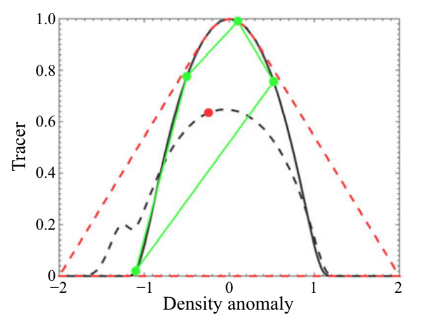
\includegraphics{figures/fig8_Jared.PNG}
            \caption{Diagramme de dispersion issus de \cite{penney_diapycnal_2020}. L'advection ne modifie pas le nuage de point mais peut rapprocher des particules fluides avec des propiétés différentes, comme les quatres particules vertes. Le mélange homogénéisera les caractéristiques densité-traceur des parcelles à l'intérieur d'une cellule dont la taille est déterminée par le coefficient de diffusion. Les caractéristiques densité-traceur résultantes de cette cellule sont alors les valeurs moyennes des propriétés initiales, pondérées par leur rapport volumétrique (par exemple le point rouge). Cela implique que le nuage de points après advection et mélange sera contenu dans l'enveloppe convexe de la distribution initiale (région à l'intérieur de la courbe en pointillés rouges).}
        \end{figure}
        
        Dans cette étude, les conditions pour valider cette propriété ne sont plus valides. Comme les coefficients de diffusion de densité et traceur ne sont plus les mêmes, il n'y a plus de déterminisme entre traceur et densité.
    
    
        \subsubsection{Réarrangement isopycnal}
        
        Le réarrangement isopycnal est un formalisme pour visualiser l'évolution macroscopique de l'instabilité en trouvant, de manière conservative, un profil vertical 1D à partir du domaine 3D. Il a été introduit par \citep{nakamura_two-dimensional_1996} et \citep*{winters_diascalar_1996} pour des écoulements spatialement inhomogènes où les traceurs sont advectés et diffusés. \\
        \newline
        Article Jared : \textit{Contours (in two dimensions) or surfaces (in three dimensions) of tracer concentration are used to define coordinate surfaces or contours, but the latter are labelled not by the value of the tracer concentration but the area (in two dimensions) or volume (in three dimensions) enclosed by the surface. If the tracer has some kind of geometric organisation, then the coordinate system and the variation of tracer concentration within that system represent that organisation. For the KH instability and for other flows in density-stratified fluids, the natural tracer is the density and the corresponding tracer-based coordinate, z\∗, represents a vertical coordinate. \\
        Note that the rearranged (or background) density field ρ∗(z∗, t) may be calculated from the 3-D simulation by rearrangement to construct a monotonic profile. That is, fluid elements, each with a specified infinitesimal volume, are ordered by their density, giving density as a function of cumulative volume (i.e. the volume of fluid with density less than a given value), and then the volume is converted to a vertical coordinate z\∗ by dividing by the horizontal area of the fluid domain. The coordinate z∗ is then a decreasing function of ρ\∗. The value of z\∗ for a given ρ∗ is therefore proportional to the integral, down to ρ\∗ of the weight defined previously in § 4.1. (Note that, typically, (5.1) is written in terms of ρ and z\∗ (for example, Smyth et al. 2005), with ∂ρ/∂z∗ implicitly referring to the adiabatic rearrangement of the density field. For clarity, ρ\∗ will be used here for density when it is being regarded as a function of z\∗, and ρ will be used when it is being regarded as a function of the Cartesian coordinates (x, y,z), such as in the numerator of the right-hand side of (5.2).)}
        \newline
        Ce réarrangement isopycnal est en faite une représentation macroscopique des processus petites-échelles. Il a l'avantage d'être conservatif, c'est-à-dire de ne pas modifier les propriétés des particules, le terme de réarrangement adiabatiques est souvent utilisé dans la littérature. C'est le seul moyen connu d'obtenir un profil macroscopique sans rajouter de processus non conservatif (diabatique) contrairement à une moyenne spatiale qui, par définition, homogénéise les propriétés sur un espace donné. \\
        Le profil obtenu issu du réarrangement de la densité est le profil de plus basse énergie potentielle et il ne varie au cours du temps qu'avec des processus non conservatif, i.e avec le mélange (\cite*{winters_diascalar_1996}. --> extraction du mélange diffusif et convectif (pour des fluides incompressibles winter et d'asaro)
        
        
        \subsubsection{Diffusion effective}
        
        La diffusion effective est la diffusion efficace à l'échelle macroscopique. Or l'évolution du profil macroscopique (issu du réarrangement isopycnal) peut être écrite sous la forme d'une équation de diffusion (\citep{penney_diapycnal_2020-1}): 
        \begin{equation}
            \label{rho*}
            \frac{\partial\rho_*}{\partial t}=\frac{\partial}{\partial z_*}(K_{\rho}\frac{\partial\rho_*}{\partial z_*})
        \end{equation}
        Avec $K_{\rho}$ la diffusion effective, seule inconnue de cette équation, l'évolution de $\rho_*$ nous est donnée par le réarrangement isopycnal de la sortie de la simulation. D'après l'annexe C de \citep{penney_diapycnal_2020}, la diffusion effective s'écrit sous la forme :
        \begin{equation}
            \label{Keff}
            \frac{K_{\rho}}{\kappa_{\rho}}=\frac{\langle\vert\Delta\rho\vert^2\rangle_{z_*}}{(\dfrac{\partial\rho_*}{\partial z_*})^2}
        \end{equation}
         ...
        
        
%----------------------------------------------------------------------------
%%  CONFIGURATION NUMÉRIQUE
%----------------------------------------------------------------------------        
\section{Configuration numérique}
    
%---Conditions initiales------------------------------------------------------    
    \subsection{Conditions initiales}
    
    Les équations sont toutes adimentionalisées par des échelles typiques des instabilités KH. Les variables dimensionnelles sont notées avec des tildes. 
    \begin{center}
       $x=\Tilde{x}/h$  \hspace{1cm}  $y=\Tilde{y}/h$  \hspace{1cm}   $z=(\Tilde{z}-z_0)/h$   \hspace{1cm}    $t=\Tilde{t}U_0/h$    \hspace{1cm}  $u=\Tilde{u}/U_{0}$    \hspace{1cm}   $\rho =( \Tilde{\rho}-\rho_0)/\Delta\rho$   \hspace{1cm}     $\phi=\title{\phi}/\Delta\phi$ \\ 
    \end{center}
    Avec $h$ la hauteur de la couche du cisaillement, $z_0$ le milieu du domaine vertical (également centre de la couche de cisaillement), $U_0$ la moitié de la variation de vitesse initiale sur le domaine, $\rho_0$ la densité médiane sur la distribution initiale de densité, $\Delta\rho$ la moitié de la variation de densité initiale sur tout le domaine et $\Delta\phi$ la concentration initiale maximale du traceur. \\
    \newline    
    \textbf{Densité} \\
    La distribution initiale de densité est linéaire, ainsi chaque particule fluide a une position unique sur le diagramme de dispersion initial :
    \begin{equation}
    \label{rho_ini}
        \rho(x,y,z,t=0)=-z\Delta\rho
    \end{equation}
    Le choix de la stratification, $\Delta\rho$, affecte le nombre de Richardson. Dans cette étude $\Delta\rho=1.2$ est assez faible pour avoir un $Ri=4.5\ 10^{-3}<< 1/4$. Cependant, si la stratification venait à augmenter, le nombre de Richardson dépasserait difficilement la valeur de 1/4 avec une telle configuration (Figure \noparref{TG_deltarho}). Il en est de même pour la longueur d'onde la plus instable,  d'après la théorie de Taylor-Golstein, elle ne varie que très peu avec $\Delta\rho$ dans cette étude. \\
    \begin{figure}[!h]
	\centering		
		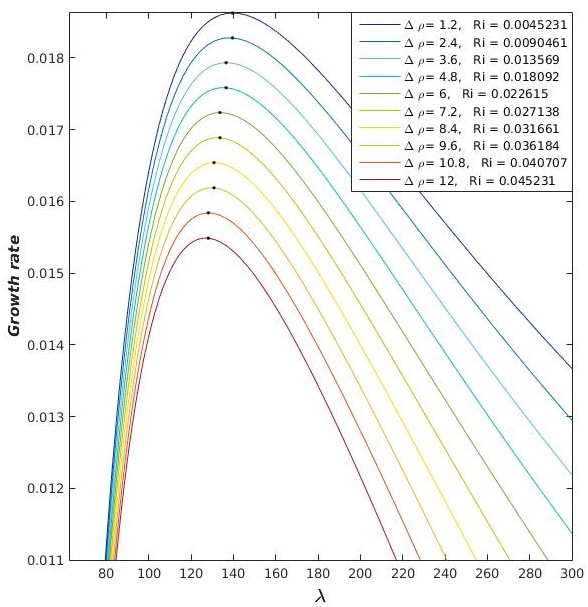
\includegraphics[width=0.55\linewidth]{figures/TG_delatrho.jpg}
\caption[Taylor-Goldstein]{\textit{Prédiction du taux de croissance en fonction de la longueur d'onde d'après la théorie de Taylor-Goldstein pour plusieurs gammes de stratifications}}
	\label{TG_deltarho}
\end{figure}
    \newline
    \textbf{Vitesse} \\
    Le champ de vitesse initiale est : 
    \begin{subequation}
    \begin{align}
        \displaystyle
            \label{u_ini}
            & u(x,y,z,t=0)=U(z)+u'(x,y,z) \\
            \label{v_ini}
            & v(x,y,z,t=0)=v'(x,y,z) \\
            \label{w_ini}
            & w(x,y,z,t=0)=w'(x,y,z)
    \end{align}
    \end{subequation}
    $U(z)$ est le cisaillement vertical de vitesse initial. Il est sous la forme d'une tangente hyperbolique centrée,
    \begin{equation}
        \label{u0_ini}
        U(z)=-tanh(z)
    \end{equation}
    ainsi la couche supérieure va vers la gauche et la couche inférieure vers la droite avec la même vitesse. $u', v'$ et $w'$ sont les petites perturbations nécessaires pour enclencher l'instabilité. Leur forme est choisie pour que le champ de vitesse initiale soit non divergent.
    \begin{subequation}
        \begin{align}
        \displaystyle
            \label{u'_ini}
            & u'(x,y,z)=\epsilon f'(z)\sin{(\frac{2\pi n_x}{L_x}x)}(1+\epsilon_{3D}\sin{(\frac{2\pi n_y}{L_y}y)}) \\
            \label{v'_ini}
            & v'(x,y,z)=0 \\
            \label{w'_ini}
            & w'(x,y,z)=-\epsilon f(z)\frac{2\pi n_x}{L_x}\cos{(\frac{2\pi n_x}{L_x}x)}(1+\epsilon_{3D}\sin{(\frac{2\pi n_y}{L_y}y)})
        \end{align}
    \end{subequation}
    La fonction $f(z)$ localise la perturbation initiale dans la région du cisaillement : 
    \begin{equation}
        f(z)=1-tanh^2(z)
    \end{equation}
    %\[f(z)=1-tanh^2(\frac{z}{\alpha})\]
    %Avec $\alpha=4.29$ et $\epsilon=0.01$
    Avec $\epsilon=0.01$ pour un paramètre sans dimension qui définit l'amplitude de la perturbation dans le sens du courant et $\epsilon_{3D}=0.2$ l'amplitude transverse. $n_x$ et $n_y$ définissent respectivement les longueurs d'ondes dans la direction x et y. \\
    \newline
    \textbf{Traceur passif} \\
    Le traceur passif est concentré dans la couche de cisaillement avec une forme :
    \begin{equation}
    \label{phi_ini}
        \phi(x,y,z,t=0)= a\Delta\phi sech^2(az-b)
    \end{equation}
    Avec les constantes $a=1$, qui contrôle l'épaisseur de la couche initiale, et $b=0$, qui contrôle la position de la couche de traceur par rapport au milieu vertical du domaine. 
    
%---Paramètres numériques-----------------------------------------------------    
    \subsection{Paramètres numériques}
    
    Choix de la grille, des pas de temps
    Toutes les simulations présentées ici ont les mêmes conditions initiale sur la structure de la densité, du traceur et du champ de vitesse. Les nombres sans dimensions sont également constants, Ri=0.0045 (sans dimension ?) et Re=2000. La longueur d'onde sans dimension la plus instable prévu par la théorie de Taylor-Godstein dans ces conditions est $\lambda_{KH}=14.0$. La longueur du domaine est choisie telle que $L_x\approx \lambda_{KH}$ pour n'avoir qu'un seul vortex qui se forme. Les nombres de points de grille ($N_x$, $N_y$ et $N_z$ respectivement dans les directions x, y et z) sont choisis pour avoir une résolution sans dimension isotrope : $\Delta x=\Delta y=\Delta z=0.055$. Les paramètres numériques sont résumés dans le tableau :
    \begin{center}
    \begin{tabular}{|c|c|c|c|c|}
    \hline
         Domaine &  Grille & Pas de temps & Pas de temps NBQ & $C_s$ \\ \hline
         $L_x = 14.0$ & $N_x = 256$ & & &\\
         $L_y = 5.3$  & $N_y = 96$  & \Delta t = 0.006 & $N\Delta_{FAST} = 10$ & $C_s=10$ \\
         $L_z = 28.6$ & $N_z = 512$ & & & \\
         \hline
    \end{tabular}
    \end{center}
%---Tests numériques----------------------------------------------------------    
    \subsection{Tests numériques}
    
    Une série de tests en 2D a permis de valider la configuration utilisée dans cette étude. Dans un premier temps, j'ai évalué la diffusion implicite du schéma numérique 
    kappa net (diffusion implicite+explicite) on ne peut pas descendre les diffusions mol en dessous de la diffusion numérique. \\
    Test vitesse acoustique \\
   
%---Liste des simulations----------------------------------------------------------     
    \subsection{Liste des simulations}
    
    \begin{center}
    \begin{tabular}{|c|c|c|c|c|}
    \hline
         N simulation & $\kappa_{\rho}$ & $\kappa_{\phi}$ & $\kappa_{\rho}/\kappa_{\phi}$ \\ \hline
         $1$ & $5.10^{-3}$ & $5.10^{-3}$ & $1$\\
         \hline
         $2$ & $5.10^{-2}$ & $5.10^{-3}$ & $10$ \\
         \hline
         $3$ & $5.10^{-1}$ & $5.10^{-3}$ & $100$\\
         \hline
         $4$ & $5.10^{-3}$ & $5.10^{-2}$ & $0.1$\\
         \hline
         $5$ & $5.10^{-3}$ & $5.10^{-1}$ & $0.01$\\
         \hline
    \end{tabular}
    \end{center}
    Variation de krho et kphi


%----------------------------------------------------------------------------------
%%   RESULTATS
%----------------------------------------------------------------------------------
\newpage
\section{Résultats}

  \subsection{Variation du coefficient de diffuison de la densité}
  
    \subsubsection{Évolution de la densité et du traceur}

    \begin{figure}[h]
    %\hfill
        \centering
        \label{rhodiff}
        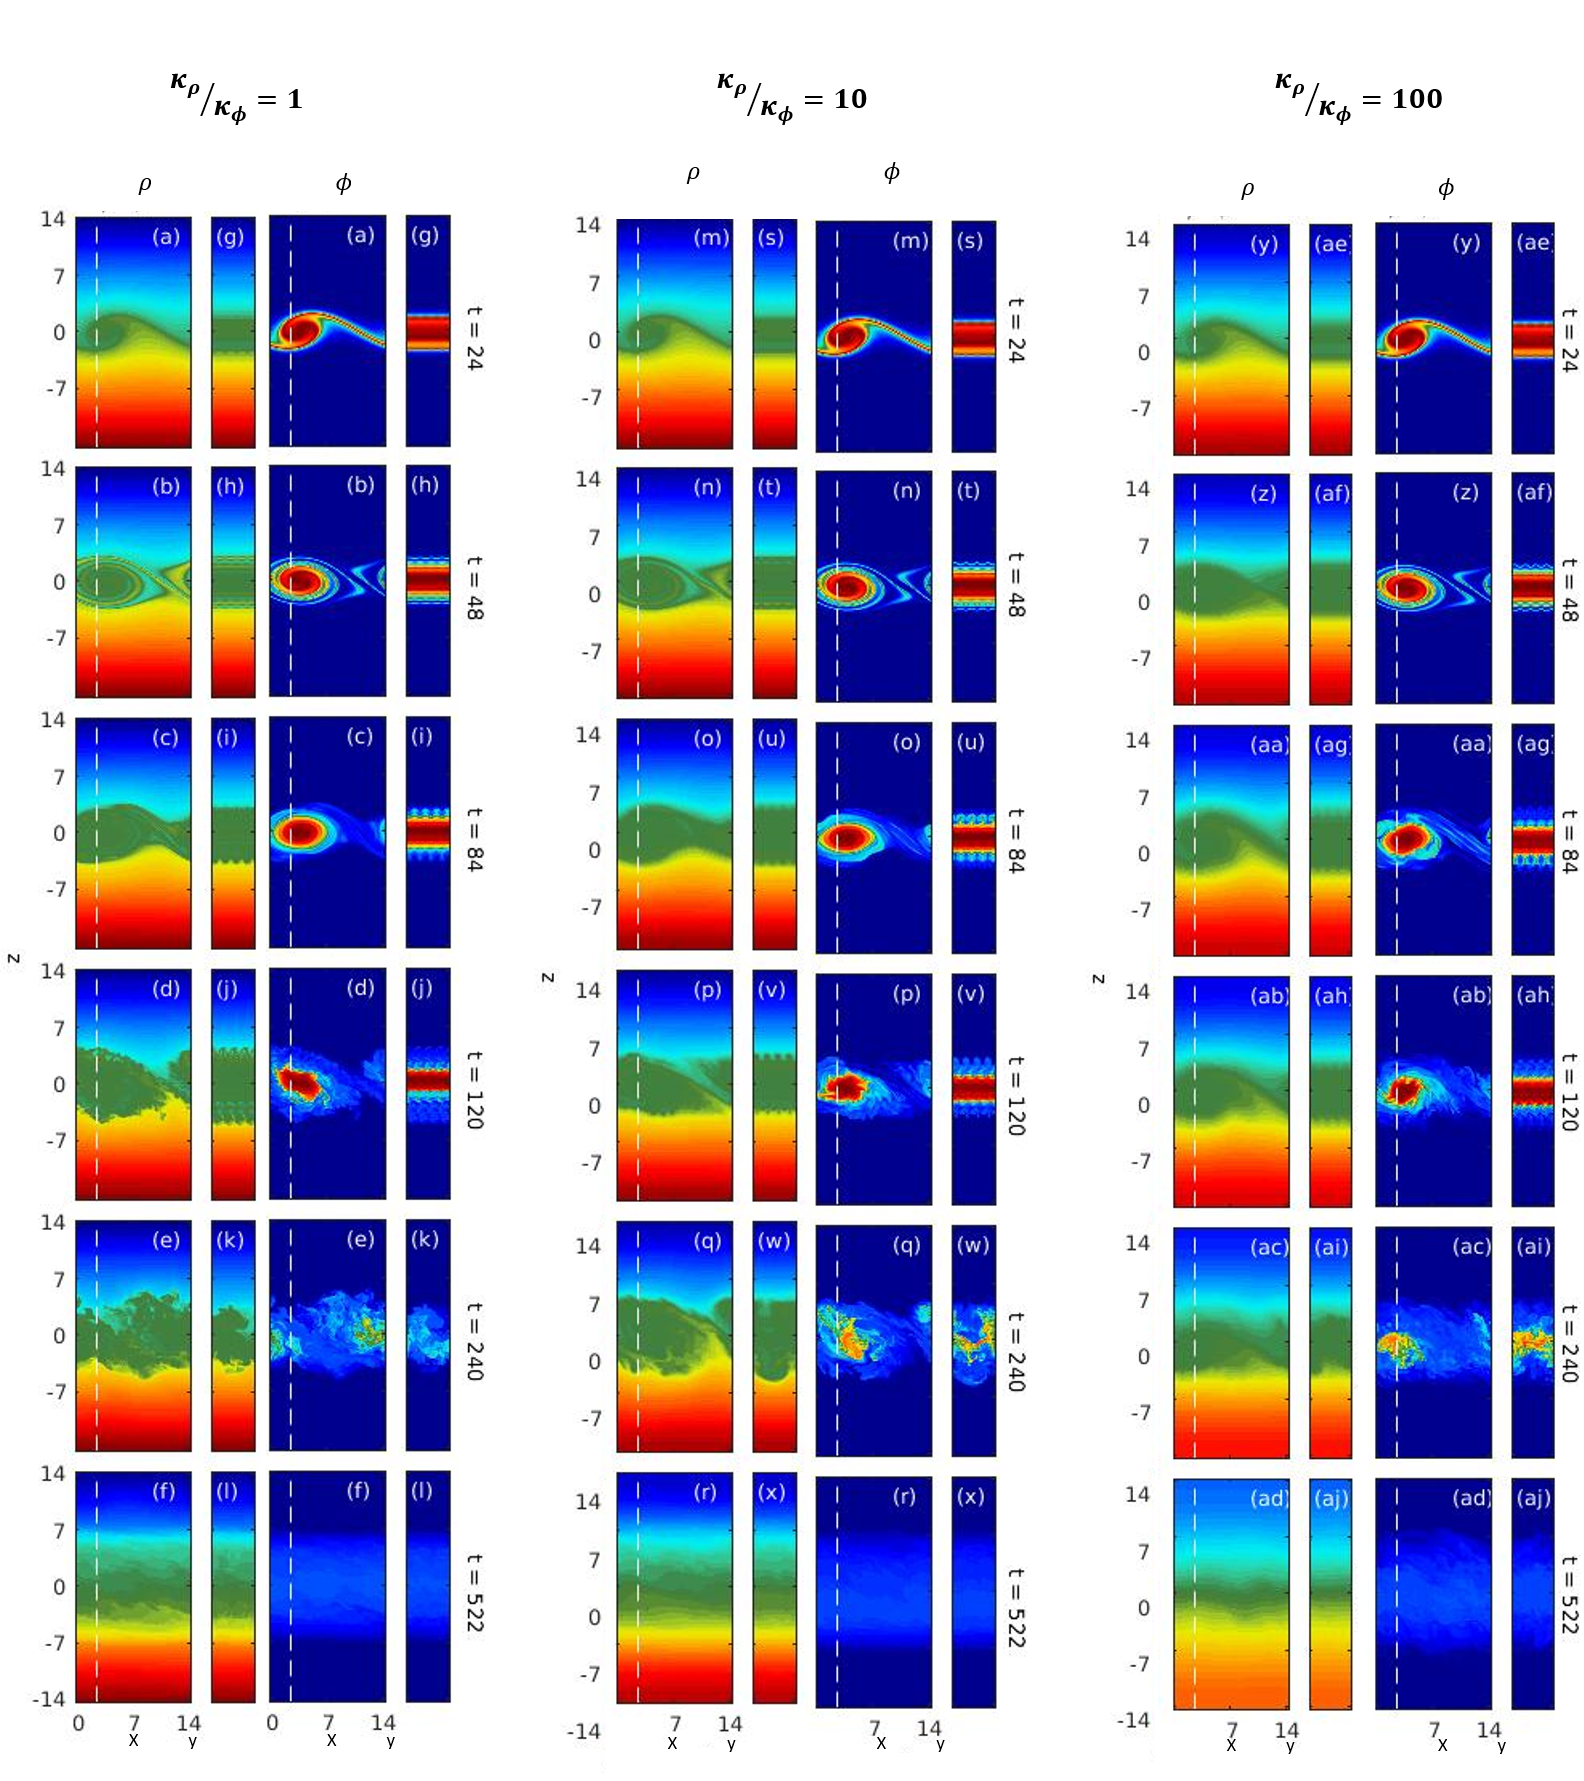
\includegraphics[width=0.95\linewidth]{figures/rhodiff.png}
        \caption{Légende}
    \end{figure}
    
    \begin{figure}[!h]
    %\hfill
        \centering
        \label{scatterplot_rho}
        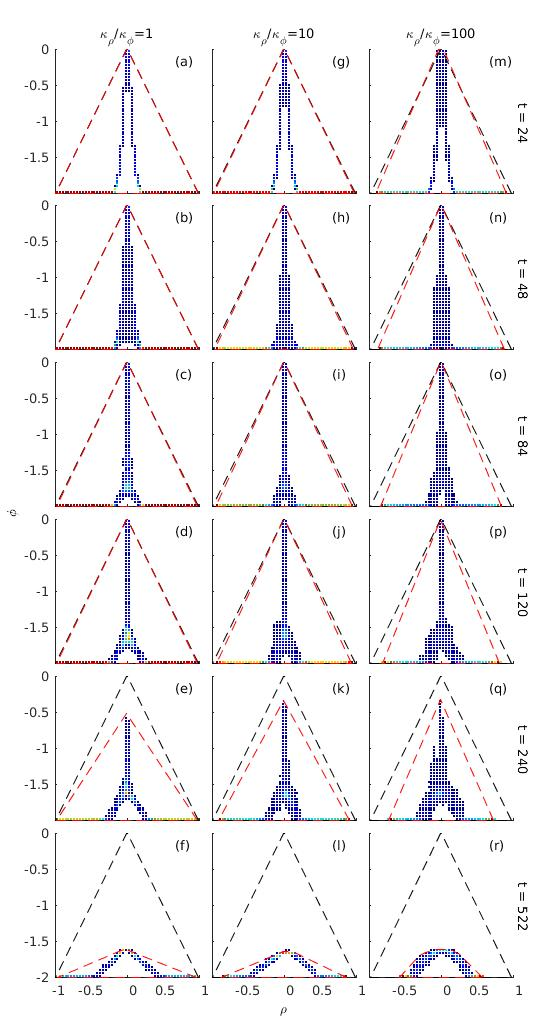
\includegraphics[width=0.6\linewidth]{figures/scatterplot_rhodiff.jpg}
        \caption{Légende}
    \end{figure}
    
    La figure \noparref{rhodiff} présente des coupes z-x et z-y pour la simulation de références (cas 1) ou les coefficients de diffusion de la densité et du traceur sont les mêmes, et pour les simulations ou le coefficient de diffusion de la densité est 10 fois supérieur (cas 2), puis 100 fois supérieur (cas 3) à celui du traceur. À la première observation, même si l'évolution générale de la densité et du traceur semble proche, on voit que l'instabilité dynamique est modifiée avec le coefficient de diffusion de la densité. Sur la figure ??? on a les diagrammes de dispersion aux mêmes pas de temps. À t=24, le diagramme de dispersion de la simulation de référence est proche de son état initial, ce qui veut dire que les particules sont seulement advectées de manière adiabatique (conservative). Le pic correspond à la couche centrale de traceur, et sa largeur indique la pénétration du traceur dans les gammes de densités. Initialement, la majorité des particules fluides sont neutres en traceur, elles sont localisées à la base du diagramme de dispersion ($\phi=0$). Pour le cas 2 et 3 on note des signes de faible processus diabatique (non conservatif) liés à la diffusion lente plus élevée dans ces deux simulations. Le vortex caractéristique des instabilités de KH se forme dans la zone de cisaillement et étire les surfaces isopycnales, ce qui favorise le mélange non conservatif. Sur les diagrammes de dispersion, on voit bien ce mélange diabatique à t=48 avec un étalement du nuage de point. Ensuite des instabilités transverses se mettent en place, on commence à les voir sur les coupes z-y de la figure ??? à t=84. À t=120, les instabilités transverses et convectives décomposent rapidement le vortex et favorisent une homogénéisation rapide en traceur et densité. Au niveau des diagrammes de dispersion, on voit ce mélange qui réduit le pic lié à la couche centrale concentrée en traceur à t=240. On note aussi qu'un noyau central concentré en traceur s'est formé à la fois sur la figure ??? et sur les diagrammes de dispersion. Le mélange non conservatif et la dissipation continuent de faire effet jusqu'à dissiper l'instabilité. Même si les étapes sont similaires pour les trois cas, on voit bien que les profils finaux sont différents. Sur la figure ??? le traceur semble s'homogénéiser moins bien pour le cas 3 alors que le gradient de densité est beaucoup plus faible, la couche centrale n'est presque plus marquée. Pour les cas 1 et 2, la couche centrale s'est élargie verticalement en homogénéisant ses propriétés en densité et traceur. On note des différences sur les diagrammes de dispersion également. Pour le cas 1 on retrouve la forme linéaire par morceau décrite par \cite{penney_diapycnal_2020} avec du traceur dans des nouvelles gammes de densité. Pour le cas 2 on retrouve également cette forme mais avec un pic qui semble plus étalé donc avec du traceur dans des gammes de densité plus grandes que le cas 1. Enfin, pour le cas 3 on ne retrouve pas le même comportement, le nuage de point ne devient pas aussi compacte que pour les autres cas et un plateau s'est créé au sommet du pic alors qu'il semble moins étalé en densité. Pour ce dernier cas, on a donc moins d'étalement du traceur, mais les particules affectées sont plus homogènes.
    
    \subsubsection{Évolution macroscopique}
    
    À partir des sorties des simulations précédentes, le profil macroscopique de la densité et du traceur passifs, issu de l'équation ???, sont calculés à chaque pas de temps (Figure \noparref{rhodiff_star}). Pour les trois simulations, on retrouve les deux phases de mélange à $t\approx50$ quand le vortex s'enroule et à $t\approx250$ quand les instabilités transverses apparaissent. Pour la densité, dans les cas 1 et 2 (Figure \noparref{rhodiff_star}a-b), ces deux évènements se traduisent par un étalement vertical de la couche centrale ($\rho\approx 0$) alors que pour le cas 3(Figure \noparref{rhodiff_star}c), les instabilités transverses semble faire disparaitre cette couche centrale. La couche centrale en traceur passif (Figure \noparref{rhodiff_star}d-e-f) augmente progressivement pour les trois cas, mais le mélange homogénéise significativement la couche à partir de $t\approx 250$ dans les trois cas. 
    \\
    \begin{figure}[!h]
    %\hfill
        \centering
        \label{rhodiff_star}
        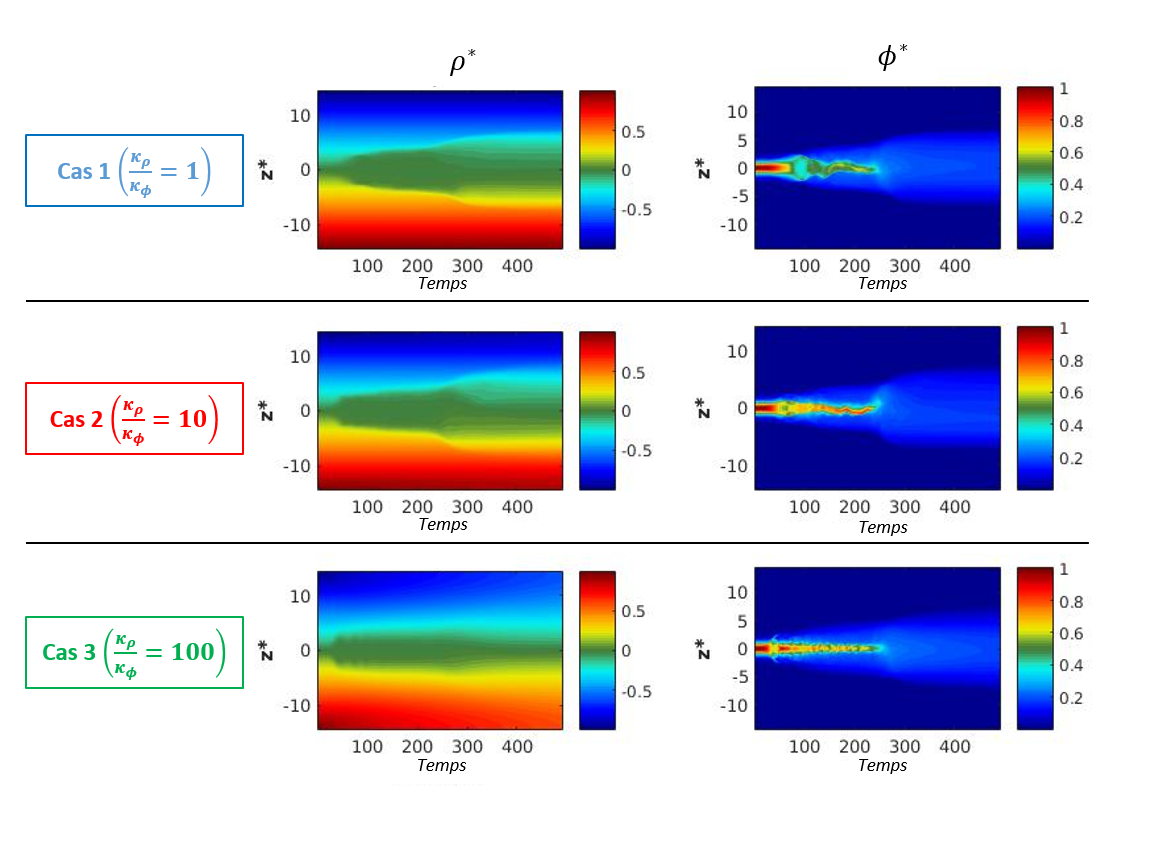
\includegraphics[width=0.9\linewidth]{figures/rhodiff_star.png}
        \caption{Légende}
    \end{figure}
    Pour mieux analyser l'influence du mélange sur les profils macroscopiques, les profils finaux issu du réarrangement sont tracés en trait plein sur la figure \noparref{rhodiff_profils_Krho}. La densité, pour le cas 1 et 2, a formé une couche centrale autour de $\rho\approx0$ alors que dans le cas 3 on ne distingue pas cette couche. Les interactions avec la surface et le fond modifient les profils finals avec l'augmentation du coefficient de diffusion (cas 2 et 3). Dans le cas 3 cette interaction est très marquée et pourrait donc avoir un impact sur la dynamique au centre de la colonne d'eau. Pour le traceur, on note un léger étalement vertical avec l'augmentation du coefficient de diffusion de la densité.\\ 
    En trait pointillé sont tracés les profils virtuels calculés avec une simple équation de diffusion macroscopique utilisant le coefficient de diffusion effectif (equation ???). On cherche à savoir si c'est profils virtuels peuvent prédire l'évolution de la densité et du traceur. Comme attendu, pour la densité, les profils virtuels finaux sont similaires aux profils macroscopiques. Le profil du traceur est prédit par le profil virtuel seulement dans le cas 1, ce qui est cohérent avec \cite{penney_diapycnal_2020}. À partir du moment ou les coefficients de diffusion de la densité et des traceurs sont différents, on ne retrouve pas les profils macroscopiques à partir de l'évolution virtuelle. 
    
    \begin{figure}[!h]
    %\hfill
        \centering
        \label{rhodiff_profils_Krho}
        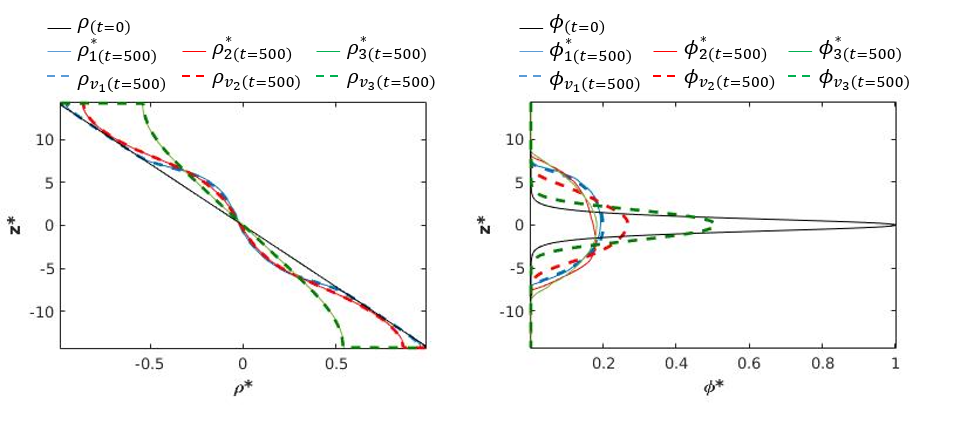
\includegraphics[width=1\linewidth]{figures/rhodiff_profils_Krho.png}
        \caption{Légende}
    \end{figure}
    
    
  \subsection{Variation du coefficient de diffusion du traceur passif}
  
    \subsubsection{Évolution de la densité et du traceur passif}
    
    \begin{figure}[!h]
    %\hfill
        \centering
        \label{phidiff}
        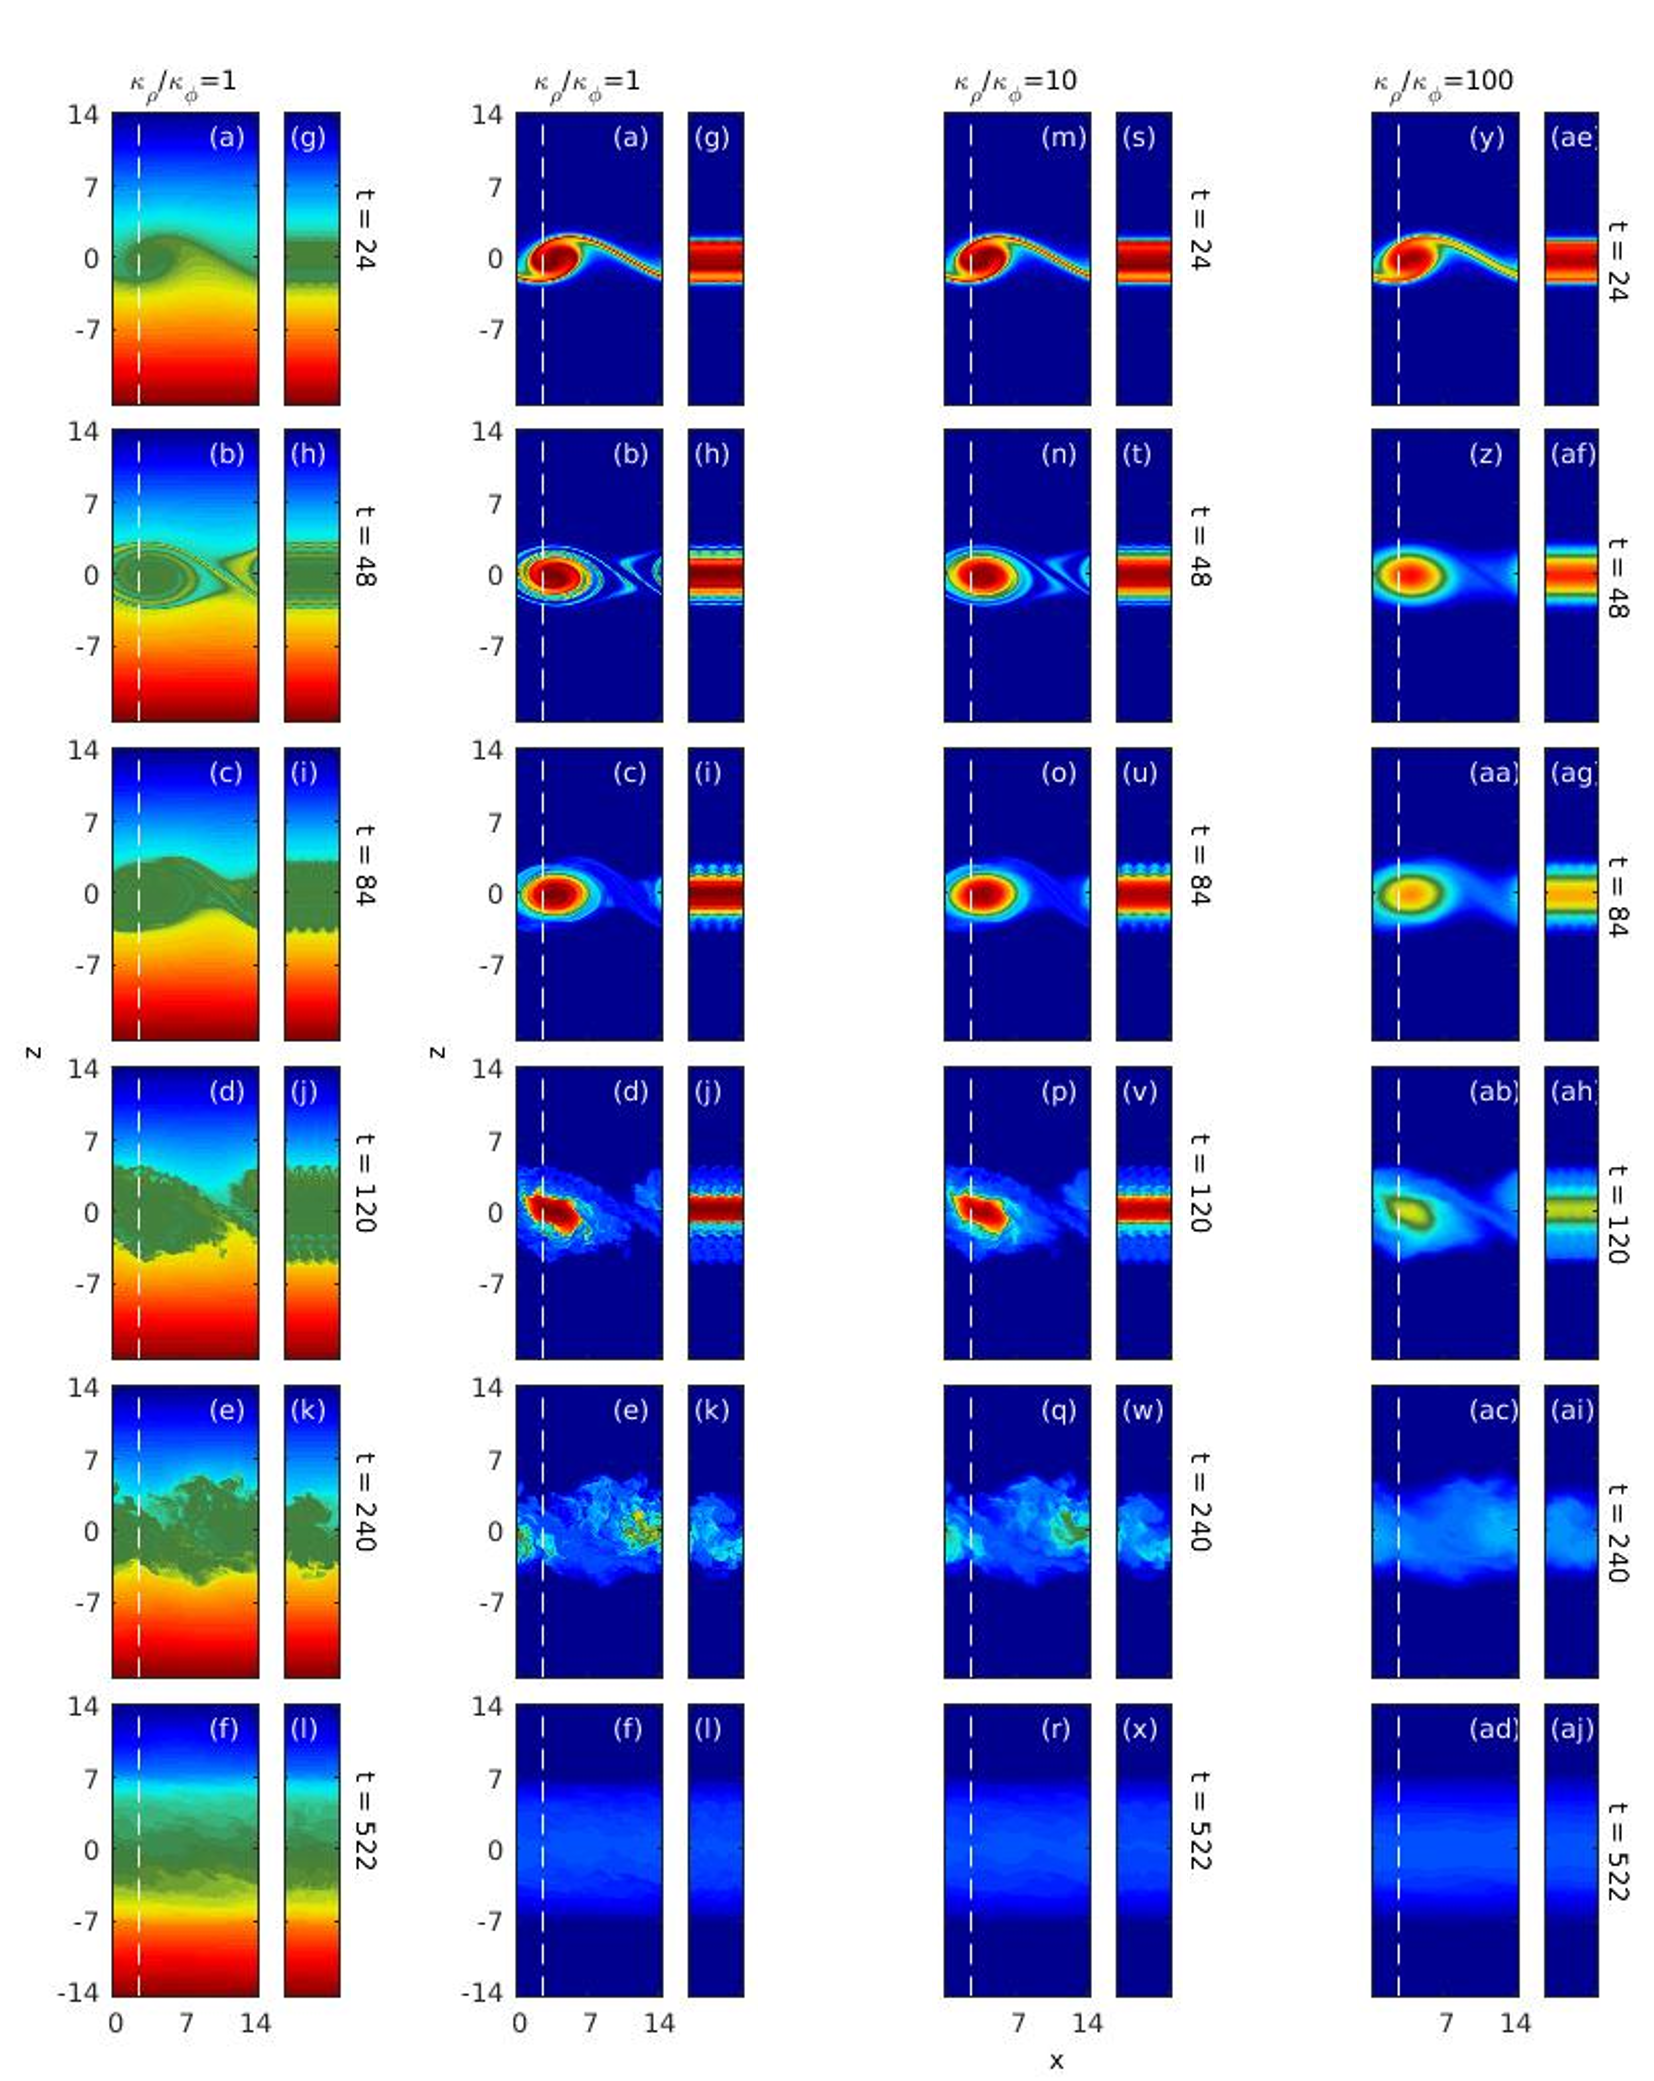
\includegraphics[width=0.95\linewidth]{figures/phidiff.png}
        \caption{Légende}
    \end{figure}
    
    \begin{figure}[!h]
    %\hfill
        \centering
        \label{scatterplot_phi}
        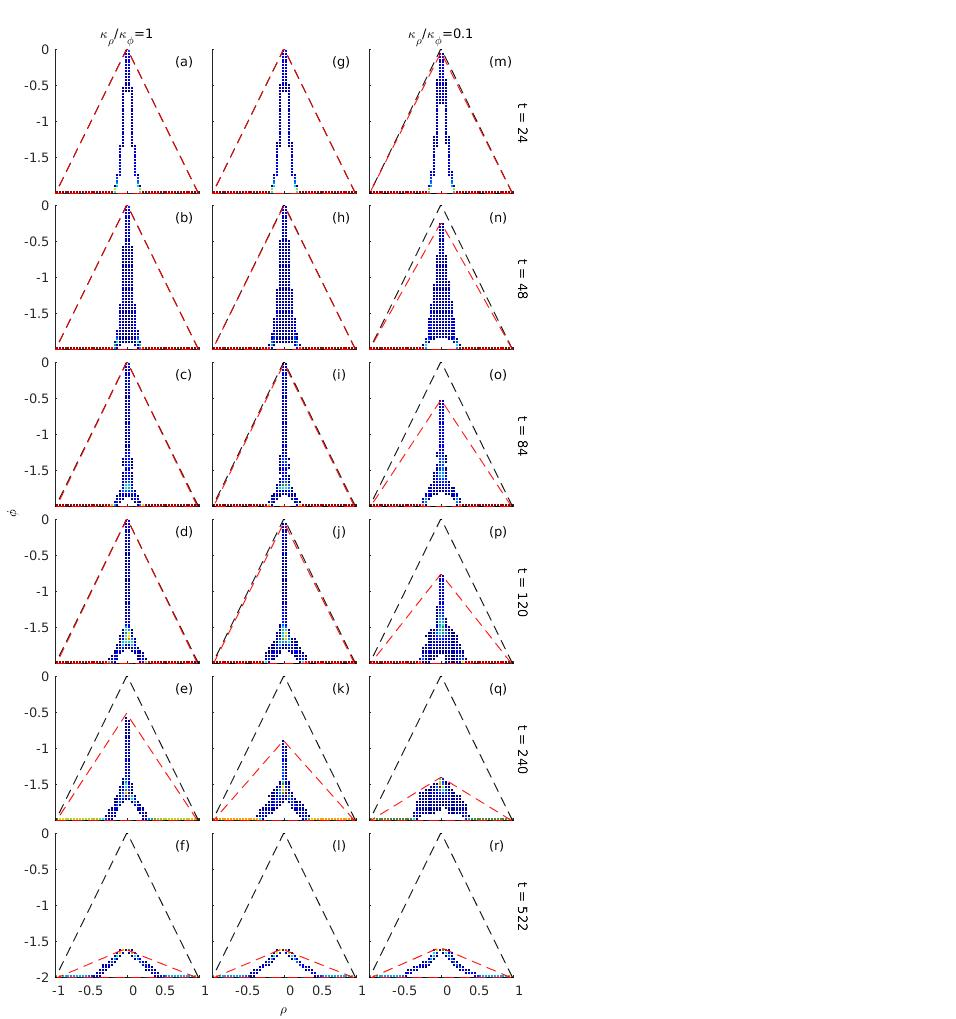
\includegraphics[width=1.3\linewidth]{figures/scatterplot_phidiff.jpg}
        \caption{Légende}
    \end{figure}
    
    La variation du coefficient de diffusion du traceur n'affecte pas la dynamique, car le traceur est passif. L'évolution de l'instabilité est donc la même que celle décrite dans la partie ??? pour le cas 1. Cependant, l'homogénéisation des particules en traceur est affectée, car on modifie le rayon d'action des particules fluides, mais il est difficile de voir une différence entre les profils finaux des trois cas présentés sur la figure ???. Pour ce qui est des diagrammes de dispersions (figure ???), on note une diminution plus rapide du pic avec l'augmentation du coefficient de diffusion du traceur passif, ce qui traduit un lissage des concentrations extrêmes en traceur plus efficace. Les nuages de points finaux sont sensiblement similaires avec une forme linéaire par morceaux.
    
    \subsubsection{Évolution macroscopique}
    
    \begin{figure}[!h]
    %\hfill
        \centering
        \label{scatterplot_phi}
        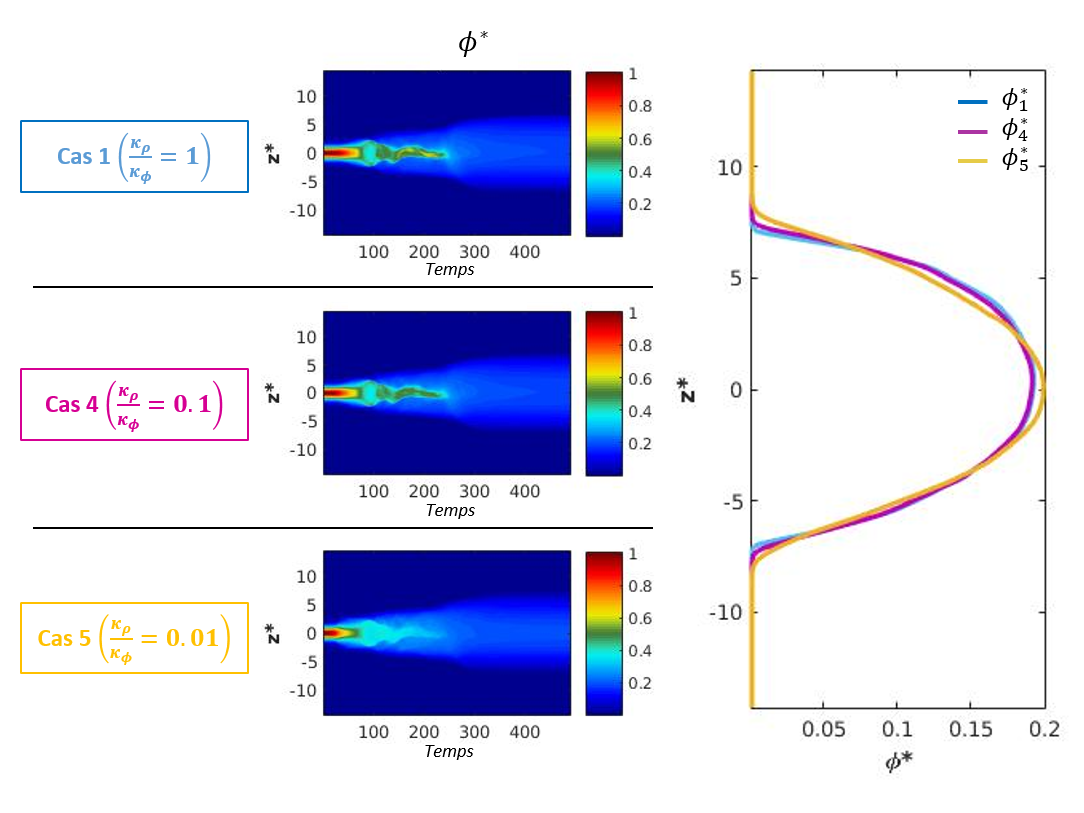
\includegraphics[width=1\linewidth]{figures/phidiff_star.png}
        \caption{Légende}
    \end{figure}
    
  \subsection{Variation de la position ?}



%----------------------------------------------------------------------------------
%%   DISCUSSION
%----------------------------------------------------------------------------------
\newpage
\section{Discussion}

Rupture du comportement \\
Détermination de Keff pour le traceur \\
sensibilité à la position \\
différence entre strat en S ou T \\
Augmentation de la viscosité --> echelle de Kolmogorov et echelle de diffusion ?

%----------------------------------------------------------------------------------
%%   CONCLUSION
%----------------------------------------------------------------------------------

\section{Conclusion}

\bibliographystyle{apalike}
\bibliography{StageM2}
%citep %citet

\end{document}